\documentclass[sigconf,natbib=true,anonymous=true]{acmart}

%% Submission-time hygiene -------------------------------------------------
\settopmatter{printacmref=false}     % suppress ACM Reference Format box
\setcopyright{none}                  % no copyright block in anonymous submission
\renewcommand\footnotetextcopyrightpermission[1]{}
\acmConference[CIKM '26]{Proceedings of the 35th ACM International
  Conference on Information and Knowledge Management}{November 7--11,
  2026}{Rome, Italy}
\acmYear{2026}
\acmISBN{}
\acmDOI{}

%% Optional packages -------------------------------------------------------
\usepackage{booktabs}
\usepackage{amsmath}
\usepackage{graphicx}
\usepackage{tikz}
\usetikzlibrary{positioning, arrows.meta, shapes.geometric,
                fit, backgrounds, calc}

\begin{document}

\title{Universal Pathologies, Conditional Consequences:
  A Triple-Robustness Analysis of RAG for Multi-Hop Traceability}

%% Double-blind anonymized author block for CIKM 2026 submission.
%% acmart's `anonymous=true' (in \documentclass options) suppresses these
%% fields in the rendered PDF. For ArXiv camera-ready, switch back to:
%%   \author{Meftun Akarsu} ... Technische Hochschule Ingolstadt ...
%%   \author{Burak \"Ozdemir} ... Independent Researcher, Ankara, Turkey
\author{Anonymous Author(s)}
\affiliation{%
  \institution{Anonymous Institution}
  \country{}
}

\begin{abstract}
Multi-hop traceability over typed requirement graphs is a
safety-critical retrieval problem in regulated domains such as
DO-178C aerospace software certification. Existing approaches address
parts of this problem in isolation: Adaptive-RAG routes by query
complexity but is hop-blind and graph-blind; Microsoft GraphRAG
exploits graph structure but is non-agentic; LiSSA performs single-shot
retrieval-augmented generation for traceability without typed-graph
reasoning. We propose a \emph{hop-adaptive, link-type-aware agentic}
retrieval architecture that (i)~routes queries among four retrieval
pipelines based on a query-conditioned hop-distance estimator and
(ii)~exposes a typed-edge graph-lookup tool inside an agentic critic
loop, exploiting DO-178C edge semantics
(\textit{derives\_from}, \textit{satisfies}, \textit{references},
\textit{traces\_to}) for retrieval reranking. We evaluate on a
1{,}132-row synthetic DO-178C corpus with 300 hop-stratified queries,
two-judge bias controls, BCa bootstrap confidence intervals, and a
200-query MuSiQue cross-evaluation for external validity.
[PLACEHOLDER: headline result --- e.g., adaptive routing matches the
best fixed pipeline per stratum at $X\%$ of cost, $p<0.05$ under Holm
correction.] Code and data are released for reproducibility.
\end{abstract}


%% --- ACM CCS concepts --------------------------------------------------
\begin{CCSXML}
<ccs2012>
  <concept>
    <concept_id>10002951.10003317.10003331</concept_id>
    <concept_desc>Information systems~Retrieval models and ranking</concept_desc>
    <concept_significance>500</concept_significance>
  </concept>
  <concept>
    <concept_id>10010147.10010178.10010179.10010181</concept_id>
    <concept_desc>Computing methodologies~Question answering</concept_desc>
    <concept_significance>300</concept_significance>
  </concept>
  <concept>
    <concept_id>10011007.10011074.10011076</concept_id>
    <concept_desc>Software and its engineering~Requirements analysis</concept_desc>
    <concept_significance>300</concept_significance>
  </concept>
</ccs2012>
\end{CCSXML}

\ccsdesc[500]{Information systems~Retrieval models and ranking}
\ccsdesc[300]{Computing methodologies~Question answering}
\ccsdesc[300]{Software and its engineering~Requirements analysis}

\keywords{retrieval-augmented generation, GraphRAG, requirements
  traceability, DO-178C, MuSiQue, LLM-as-judge, kappa paradox,
  triple-robustness, embedder fragility}

\maketitle

\section{Introduction}
\label{sec:intro}

Software requirements in safety-critical domains such as aerospace are
authored as typed link graphs: each requirement \textit{derives\_from}
parent requirements, \textit{satisfies} system-level intent, and
\textit{traces\_to} verification artifacts. DO-178C compliance demands
end-to-end traceability across these typed edges, and certification
authorities increasingly require auditable chains spanning two or more
hops across modules~\cite{do178c,arp4754a,easa2025npa,faa2024airoadmap}.
A practitioner asking ``how does the air-data system feed
angle-of-attack to the flight-control computer?'' needs an answer that
walks \textit{interface} edges across modules, not a paragraph
reranked by surface-level cosine similarity.

Existing retrieval-augmented generation (RAG) systems address parts of
this problem but never the whole. Vanilla dense retrieval misses
cross-module links that share little surface vocabulary.
Adaptive-RAG~\cite{adaptiverag2024} routes queries by lexical complexity
but is hop-blind and graph-blind. Microsoft GraphRAG~\cite{graphrag2024}
and follow-ups such as LightRAG~\cite{lightrag2024},
HippoRAG~2~\cite{hipporag2_2025}, and Graph-R1~\cite{graphr1_2025}
exploit graph structure but are non-agentic and untyped.
LiSSA~\cite{lissa2025} applies single-shot RAG to traceability without
typed-graph reasoning. RAG-Critic~\cite{ragcritic2025} introduces an
agentic critic loop but is evaluated on Wikipedia rather than typed
regulatory graphs.

This paper introduces a hop-adaptive, link-type-aware agentic
retrieval architecture for requirement traceability. Our contributions
are:
\begin{itemize}
  \item A \emph{hop-adaptive router} that selects among four retrieval
    pipelines---\textit{vanilla}, \textit{agentic}, \textit{graph-walk},
    \textit{agentic+graph}---conditioned on a query-derived typed-edge
    distance estimator.
  \item A \emph{link-type-aware graph-lookup tool} that exploits
    DO-178C-style edge semantics
    (\textit{derives\_from}~$>$~\textit{satisfies}~$>$~\textit{references}
    $>$~\textit{traces\_to}) for retrieval reranking inside an agentic
    ReAct loop.
  \item A \emph{hop-stratified evaluation protocol} with two-judge bias
    controls, applied to a 1{,}132-row synthetic DO-178C corpus and
    cross-evaluated on 200 multi-hop questions sampled from
    MuSiQue~\cite{musique2022}.
\end{itemize}

[PLACEHOLDER: headline empirical claim --- e.g., ``hop-adaptive routing
matches the best fixed pipeline per stratum at lower aggregate cost
($p<0.05$, Holm corrected, Cohen's $d=Z$).''] Section~\ref{sec:related}
surveys related work; Section~\ref{sec:method} describes the method;
Section~\ref{sec:experiments} details the evaluation;
Section~\ref{sec:results} reports results; and
Section~\ref{sec:discussion} discusses limitations.

\section{Related Work}
\label{sec:related}

\subsection{Agentic and Adaptive RAG}
Self-RAG~\cite{selfrag2024} introduced reflective retrieval tokens.
CRAG~\cite{crag2024} added a corrective lightweight retrieval evaluator.
Adaptive-RAG~\cite{adaptiverag2024} routes among no-retrieval,
single-step, and multi-step retrieval based on a classifier-predicted
query complexity. Search-R1~\cite{searchr1_2025} trains the retrieving
agent to interleave search and reasoning via reinforcement learning.
RAG-Critic~\cite{ragcritic2025} adds an agentic critic loop with
iterative refinement. None of these systems condition routing on
typed-graph distance, and none expose a typed graph-lookup tool;
retrieval is treated as flat text top-$k$.

\subsection{GraphRAG Family}
Microsoft GraphRAG~\cite{graphrag2024} builds entity--relation graphs
and answers via community summaries; LightRAG~\cite{lightrag2024} and
HippoRAG~2~\cite{hipporag2_2025} reduce graph-construction cost.
Han et~al.~\cite{ragvsgraphrag2025} compare RAG and GraphRAG empirically;
GraphRAG-Bench~\cite{graphragbench2026} provides a benchmark for
\textit{when} graph structure helps. Graph-R1~\cite{graphr1_2025} trains
a graph-aware retrieval policy with RL. These systems exploit graph
structure but are non-agentic: they do not loop a critic over retrieved
evidence, and they do not condition pipeline choice on hop distance.

\subsection{RAG for Requirements Traceability}
LiSSA~\cite{lissa2025} applies single-shot RAG to source--requirement
traceability. TraceLLM~\cite{tracellm2026} and TVR~\cite{niu_tvr2025}
extend LLM-based traceability with verification feedback. Graph-RAG
for compliance~\cite{graphragcompliance2024} uses domain knowledge
graphs without an agentic loop. To our knowledge, this is the first
work to combine an agentic critic loop, a typed-edge graph tool, and
hop-stratified evaluation in the requirements-traceability setting.

\section{Method}
\label{sec:method}

\begin{figure}[t]
  \centering
  \IfFileExists{figures/architecture.pdf}
    {\includegraphics[width=\columnwidth]{figures/architecture.pdf}}%
    {%% architecture-tikz.tex --- the tikzpicture body for Figure 1.
%% Single source of truth. Consumed in two ways:
%%   (a) figures/architecture.tex (standalone) for separate compile.
%%   (b) sections/04-method.tex via %% architecture-tikz.tex --- the tikzpicture body for Figure 1.
%% Single source of truth. Consumed in two ways:
%%   (a) figures/architecture.tex (standalone) for separate compile.
%%   (b) sections/04-method.tex via \input{figures/architecture-tikz}
%%       so the figure renders inline when main.tex is compiled.
%%
%% Required preamble in the host document:
%%   \usepackage{tikz}
%%   \usetikzlibrary{positioning, arrows.meta, shapes.geometric,
%%                   fit, backgrounds, calc}

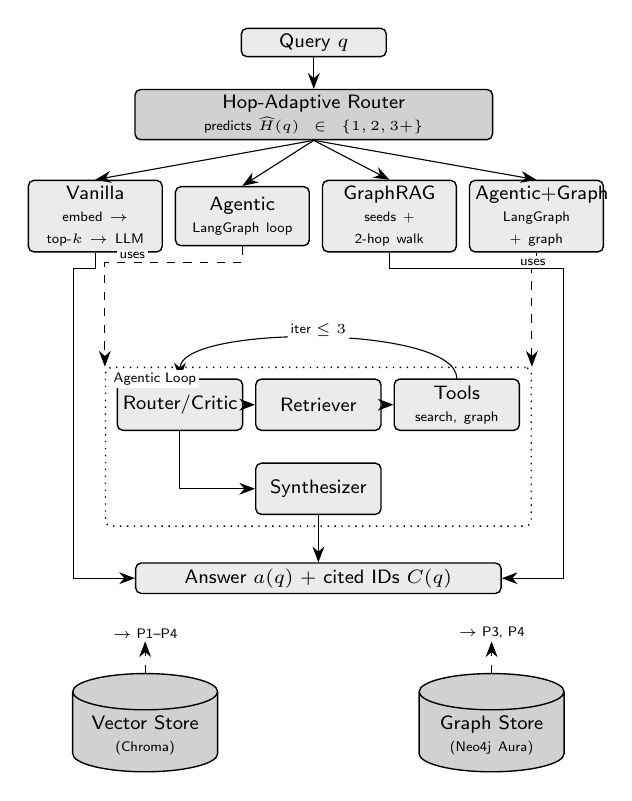
\begin{tikzpicture}[
  node distance=4mm,
  >={Stealth[length=2mm]},
  every node/.style={font=\sffamily\scriptsize}
]
\tikzset{
  box/.style    ={draw=black, line width=0.5pt, rounded corners=2pt,
                  align=center, inner sep=2pt},
  light/.style  ={box, fill=black!8},
  mid/.style    ={box, fill=black!18},
  pipe/.style   ={light, text width=1.55cm, minimum width=1.7cm,
                  minimum height=7.5mm},
  lp/.style     ={light, text width=1.45cm, minimum width=1.55cm,
                  minimum height=6.5mm},
  store/.style  ={cylinder, shape border rotate=90, aspect=0.25,
                  draw=black, line width=0.5pt, fill=black!18,
                  align=center, inner sep=2pt,
                  text width=1.7cm, minimum height=7mm},
  arr/.style    ={->, line width=0.4pt},
  darr/.style   ={arr, dashed},
  lab/.style    ={font=\sffamily\tiny, fill=white, inner sep=1pt},
  group/.style  ={draw=black, line width=0.5pt, rounded corners=2pt,
                  dotted, inner sep=4pt}
}

%% ----- Top: Query, Router -----
\node[light, text width=1.7cm] (q) at (0,0) {Query $q$};
\node[mid, below=4mm of q, text width=4.4cm] (router)
  {Hop-Adaptive Router\\{\tiny predicts $\widehat{H}(q) \in \{1, 2, 3{+}\}$}};
\draw[arr] (q) -- (router);

%% ----- Pipelines (centered at x=0) -----
\node[pipe, below=5mm of router, xshift=-2.775cm] (p1)
  {Vanilla\\{\tiny embed $\to$ top-$k$ $\to$ LLM}};
\node[pipe, right=1.5mm of p1] (p2)
  {Agentic\\{\tiny LangGraph loop}};
\node[pipe, right=1.5mm of p2] (p3)
  {GraphRAG\\{\tiny seeds + 2-hop walk}};
\node[pipe, right=1.5mm of p3] (p4)
  {Agentic+Graph\\{\tiny LangGraph + graph}};
\foreach \i in {1,2,3,4}
  \draw[arr] (router.south) -- (p\i.north);

%% ----- Agentic Loop subgraph (centered below pipelines) -----
\node[lp] (critic) at (-1.7,-4.6) {Router/Critic};
\node[lp, right=1.5mm of critic] (retr)  {Retriever};
\node[lp, right=1.5mm of retr]   (tools) {Tools\\{\tiny search, graph}};
\node[lp, below=4mm of retr]     (synth) {Synthesizer};

\draw[arr] (critic) -- (retr);
\draw[arr] (retr)   -- (tools);
\draw[arr] (tools.north) to[out=90,in=90,looseness=0.5]
  node[lab, midway, yshift=1mm] {iter $\le 3$} (critic.north);
\draw[arr] (critic.south) |- (synth.west);

\begin{scope}[on background layer]
  \node[group, fit=(critic)(retr)(tools)(synth)] (loop) {};
\end{scope}
\node[lab, anchor=north west]
  at ([xshift=2pt,yshift=-1pt]loop.north west) {Agentic Loop};

%% ----- P2, P4 -> Loop (dashed "uses"; right-angle elbows) -----
\draw[darr] (p2.south) -- ++(0,-2mm) -| (loop.north west)
  node[lab, pos=0.4, above] {uses};
\draw[darr] (p4.south) -- ++(0,-2mm) -| (loop.north east)
  node[lab, pos=0.4, above] {uses};

%% ----- Output -----
\node[light, below=6mm of synth, text width=4.5cm] (out)
  {Answer $a(q)$ + cited IDs $C(q)$};
\draw[arr] (synth.south) -- (out.north);

%% ----- P1, P3 -> Output (bypass loop on the sides) -----
\draw[arr] (p1.south) -- ++(0,-2mm) -|
  ([xshift=-4mm]loop.south west) |- (out.west);
\draw[arr] (p3.south) -- ++(0,-2mm) -|
  ([xshift=4mm]loop.south east)  |- (out.east);

%% ----- Data stores at the bottom; consolidated arrows -----
\node[store, below=10mm of out, xshift=-22mm] (s1)
  {Vector Store\\{\tiny (Chroma)}};
\node[store, below=10mm of out, xshift=22mm]  (s2)
  {Graph Store\\{\tiny (Neo4j Aura)}};

\draw[darr] (s1.north) -- ++(0,4mm)
  node[lab, anchor=south] {$\to$ P1--P4};
\draw[darr] (s2.north) -- ++(0,4mm)
  node[lab, anchor=south] {$\to$ P3, P4};

\end{tikzpicture}

%%       so the figure renders inline when main.tex is compiled.
%%
%% Required preamble in the host document:
%%   \usepackage{tikz}
%%   \usetikzlibrary{positioning, arrows.meta, shapes.geometric,
%%                   fit, backgrounds, calc}

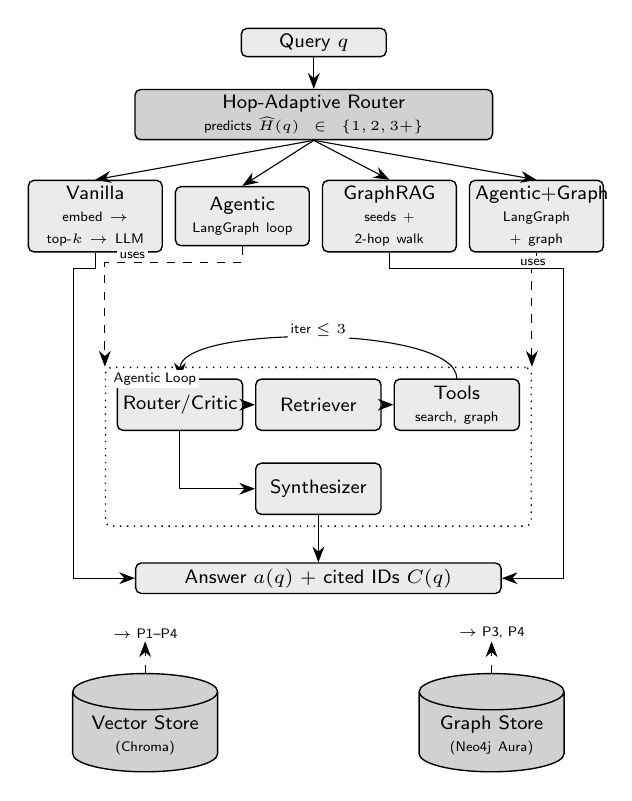
\begin{tikzpicture}[
  node distance=4mm,
  >={Stealth[length=2mm]},
  every node/.style={font=\sffamily\scriptsize}
]
\tikzset{
  box/.style    ={draw=black, line width=0.5pt, rounded corners=2pt,
                  align=center, inner sep=2pt},
  light/.style  ={box, fill=black!8},
  mid/.style    ={box, fill=black!18},
  pipe/.style   ={light, text width=1.55cm, minimum width=1.7cm,
                  minimum height=7.5mm},
  lp/.style     ={light, text width=1.45cm, minimum width=1.55cm,
                  minimum height=6.5mm},
  store/.style  ={cylinder, shape border rotate=90, aspect=0.25,
                  draw=black, line width=0.5pt, fill=black!18,
                  align=center, inner sep=2pt,
                  text width=1.7cm, minimum height=7mm},
  arr/.style    ={->, line width=0.4pt},
  darr/.style   ={arr, dashed},
  lab/.style    ={font=\sffamily\tiny, fill=white, inner sep=1pt},
  group/.style  ={draw=black, line width=0.5pt, rounded corners=2pt,
                  dotted, inner sep=4pt}
}

%% ----- Top: Query, Router -----
\node[light, text width=1.7cm] (q) at (0,0) {Query $q$};
\node[mid, below=4mm of q, text width=4.4cm] (router)
  {Hop-Adaptive Router\\{\tiny predicts $\widehat{H}(q) \in \{1, 2, 3{+}\}$}};
\draw[arr] (q) -- (router);

%% ----- Pipelines (centered at x=0) -----
\node[pipe, below=5mm of router, xshift=-2.775cm] (p1)
  {Vanilla\\{\tiny embed $\to$ top-$k$ $\to$ LLM}};
\node[pipe, right=1.5mm of p1] (p2)
  {Agentic\\{\tiny LangGraph loop}};
\node[pipe, right=1.5mm of p2] (p3)
  {GraphRAG\\{\tiny seeds + 2-hop walk}};
\node[pipe, right=1.5mm of p3] (p4)
  {Agentic+Graph\\{\tiny LangGraph + graph}};
\foreach \i in {1,2,3,4}
  \draw[arr] (router.south) -- (p\i.north);

%% ----- Agentic Loop subgraph (centered below pipelines) -----
\node[lp] (critic) at (-1.7,-4.6) {Router/Critic};
\node[lp, right=1.5mm of critic] (retr)  {Retriever};
\node[lp, right=1.5mm of retr]   (tools) {Tools\\{\tiny search, graph}};
\node[lp, below=4mm of retr]     (synth) {Synthesizer};

\draw[arr] (critic) -- (retr);
\draw[arr] (retr)   -- (tools);
\draw[arr] (tools.north) to[out=90,in=90,looseness=0.5]
  node[lab, midway, yshift=1mm] {iter $\le 3$} (critic.north);
\draw[arr] (critic.south) |- (synth.west);

\begin{scope}[on background layer]
  \node[group, fit=(critic)(retr)(tools)(synth)] (loop) {};
\end{scope}
\node[lab, anchor=north west]
  at ([xshift=2pt,yshift=-1pt]loop.north west) {Agentic Loop};

%% ----- P2, P4 -> Loop (dashed "uses"; right-angle elbows) -----
\draw[darr] (p2.south) -- ++(0,-2mm) -| (loop.north west)
  node[lab, pos=0.4, above] {uses};
\draw[darr] (p4.south) -- ++(0,-2mm) -| (loop.north east)
  node[lab, pos=0.4, above] {uses};

%% ----- Output -----
\node[light, below=6mm of synth, text width=4.5cm] (out)
  {Answer $a(q)$ + cited IDs $C(q)$};
\draw[arr] (synth.south) -- (out.north);

%% ----- P1, P3 -> Output (bypass loop on the sides) -----
\draw[arr] (p1.south) -- ++(0,-2mm) -|
  ([xshift=-4mm]loop.south west) |- (out.west);
\draw[arr] (p3.south) -- ++(0,-2mm) -|
  ([xshift=4mm]loop.south east)  |- (out.east);

%% ----- Data stores at the bottom; consolidated arrows -----
\node[store, below=10mm of out, xshift=-22mm] (s1)
  {Vector Store\\{\tiny (Chroma)}};
\node[store, below=10mm of out, xshift=22mm]  (s2)
  {Graph Store\\{\tiny (Neo4j Aura)}};

\draw[darr] (s1.north) -- ++(0,4mm)
  node[lab, anchor=south] {$\to$ P1--P4};
\draw[darr] (s2.north) -- ++(0,4mm)
  node[lab, anchor=south] {$\to$ P3, P4};

\end{tikzpicture}
}%
  \caption{Architecture. A hop-adaptive router selects among four
    retrieval pipelines based on a query-conditioned hop-distance
    estimator. Pipelines~2 and~4 share a LangGraph
    router--retriever--critic--synthesizer skeleton; the typed
    graph-lookup tool is exposed in pipelines~3 and~4. Tools
    abbreviated: \texttt{search} = \texttt{search\_documents},
    \texttt{graph} = \texttt{graph\_lookup}.}
  \label{fig:arch}
\end{figure}

\subsection{Problem Formulation}
\label{sec:problem}
We model the requirement corpus as a typed graph $G=(V,E,\tau)$ where
$V$ is the set of requirements, $E\subseteq V\times V$ is the set of
traceability links, and $\tau:E\to T$ assigns each edge a type from
$T=\{\mathrm{derives\_from},\mathrm{satisfies},\mathrm{references},
\mathrm{traces\_to}\}$. A traceability query $q$ has an unobserved hop
class $H(q)\in\{1,2,3{+}\}$ that summarizes the minimum graph distance
between the entities mentioned in $q$ and the gold answer. The system
produces an answer $a(q)$ together with cited requirement IDs
$C(q)\subseteq V$.

\subsection{Four Retrieval Pipelines}
\label{sec:pipelines}
We consider four pipelines that share an embedder, a vector store, and
a synthesizer prompt and differ only in retrieval strategy:
\textbf{(i)~Vanilla} performs dense top-$k$ retrieval over text chunks
followed by one synthesis call.
\textbf{(ii)~Agentic} runs a LangGraph
router--retriever--critic--synthesizer loop with a
\texttt{search\_documents} tool and an iteration cap of three.
\textbf{(iii)~GraphRAG} retrieves vector seeds and then walks the typed
graph for up to two hops via a Cypher query against
Neo4j, synthesizing once at the end.
\textbf{(iv)~Agentic+Graph} extends pipeline~(ii) with a
\texttt{graph\_lookup} tool node alongside \texttt{search\_documents},
allowing the critic to request typed-edge expansion when text retrieval
fails.

\subsection{Hop-Adaptive Router}
\label{sec:router}
The router predicts $\widehat{H}(q)\in\{1,2,3{+}\}$ from $q$ alone and
selects the pipeline with the best expected reward in that hop bucket
on a held-out validation set. Features include (a)~entity count via
named-entity recognition, (b)~explicit requirement-ID patterns
(regex \texttt{REQ-[A-Z]+-\textbackslash d+}), (c)~question-type cues
(e.g., \textit{trace from}, \textit{how does $X$ relate to $Y$}), and
(d)~the embedding-space norm of $q$. We instantiate two variants:
\textbf{V1}, a transparent rule-based router, and \textbf{V2}, a
multinomial logistic regressor trained on 30\% of labelled queries with
a held-out test split. Hop labels for training are obtained by walking
$G$ from gold answer chains at evaluation-set construction time.

\subsection{Link-Type-Aware Graph Tool}
\label{sec:graphtool}
The graph-lookup tool has signature
\[
  \texttt{graph\_lookup}(\mathit{seed\_ids},\,\mathit{hops},\,
                         \mathit{edge\_types})
\]
and returns chunks ranked by a hybrid score
\[
  s(c\mid q) \;=\;
    \lambda_{\mathrm{text}}\,\cos(q,c)
    \;+\; \lambda_{\mathrm{graph}}\,
          \frac{w(\tau(e_{c}))}{\mathrm{dist}(\mathit{seed},c)},
\]
where $e_c$ is the edge that brought $c$ into the candidate set,
$w:T\to\mathbb{R}_+$ assigns DO-178C-aligned semantic priorities
($\mathrm{derives\_from}>\mathrm{satisfies}>
\mathrm{references}>\mathrm{traces\_to}$), and $\lambda_{\mathrm{text}},
\lambda_{\mathrm{graph}}$ are tuned on a validation split. The tool
filters out edge types not in $T$ to avoid retrieval dilution from
auxiliary schema relations such as \textit{ALLOCATED\_TO} or
\textit{IMPLEMENTS}.

\section{Experimental Setup}
\label{sec:experiments}

\subsection{Corpus}
We use a 1{,}132-row synthetic DO-178C-style requirements corpus
spanning 32 modules (e.g., ADS, FCC, NAV, GPS, EPS, ICE) with
$\approx 3{,}000$ typed traceability edges. Synthetic generation is
necessary because certified aerospace artifacts are
intellectual-property restricted; we follow the
Synthline~\cite{synthline2025} methodology for synthetic requirements
engineering. To probe external validity we cross-evaluate on 200
multi-hop questions sampled from MuSiQue~\cite{musique2022}.

\subsection{Evaluation Queries}
We sample 300 hop-stratified queries (100 each at 1-hop, 2-hop, and
3+-hop) by walking $G$ along typed edges and surface-realising each
chain via GPT-5.4 with a constrained prompt. A 30/300 random subset
undergoes manual sanity checks. The gold tuple per query is
$(a^{\star}, C^{\star}, \tau^{\star})$---gold answer, supporting
requirement IDs, and link-type chain. A 50-query human-gold subset is
held out for judge calibration.

\subsection{Metrics}
We report RAGAS~\cite{ragas2024} faithfulness, context precision,
context recall, and answer relevancy; answer correctness against gold
IDs; cost in tokens and USD; and end-to-end latency. All metrics are
reported with hop-stratified breakdowns.

\subsection{Statistical Protocol}
The design is 5 systems $\times$ 300 queries $\times$ 3 random seeds.
We report 95\% bias-corrected and accelerated (BCa) bootstrap intervals
with 1000 resamples~\cite{jung_owen2025}, paired permutation tests
(10{,}000 permutations) for system-pair comparisons~\cite{koehn2004,
bergkirkpatrick2012}, Holm correction across the family of pairwise
contrasts, and Cohen's~$d$ effect sizes. Three seeds are adequate under
paired BCa per Jung and Owen~\cite{jung_owen2025}.

\subsection{Judge Bias Control}
Two judges score each output: GPT-5.4 (primary) and Claude-Sonnet~4
(cross-check). We report pairwise Cohen's~$\kappa$ on the 50-query
human-gold slice and a position-swap robustness check (answer~A first
versus B first) to mitigate self-preference
bias~\cite{selfpref_bias2024}. Where applicable we further compare
with established judge frameworks such as
RAGChecker~\cite{ragchecker2024} and RAGBench~\cite{ragbench2024}.

\section{Results}
\label{sec:results}

\begin{table*}[t]
  \centering
  \caption{Hop-stratified main results. Cells are mean accuracy with
    95\% BCa bootstrap CIs; $\dagger$ marks Holm-significant
    ($p<0.05$) improvement over the best non-adaptive baseline.
    [PLACEHOLDER: fill from \texttt{results/results.csv}.]}
  \label{tab:main}
  \small
  \begin{tabular}{lcccccc}
    \toprule
    System & 1-hop & 2-hop & 3+-hop & Overall & Cost (USD/q) & Latency (s) \\
    \midrule
    Vanilla                  & --- & --- & --- & --- & --- & --- \\
    Agentic                  & --- & --- & --- & --- & --- & --- \\
    GraphRAG                 & --- & --- & --- & --- & --- & --- \\
    Agentic+Graph            & --- & --- & --- & --- & --- & --- \\
    \textbf{Adaptive (ours)} & --- & --- & --- & --- & --- & --- \\
    \bottomrule
  \end{tabular}
\end{table*}

\begin{figure}[t]
  \centering
  \IfFileExists{figures/pareto.pdf}
    {\includegraphics[width=\columnwidth]{figures/pareto.pdf}}%
    {\fbox{\parbox[c][3.4cm][c]{0.92\columnwidth}{\centering\itshape
       [PLACEHOLDER: cost--quality Pareto plot] \\[2pt]
       $x$: cost/query (USD), $y$: composite quality \\[2pt]
       systems $\times$ \{low, med, high\} reasoning effort}}}%
  \caption{Cost--quality Pareto frontier across systems and
    reasoning-effort settings.}
  \label{fig:pareto}
\end{figure}

\begin{figure}[t]
  \centering
  \IfFileExists{figures/hop-curves.pdf}
    {\includegraphics[width=\columnwidth]{figures/hop-curves.pdf}}%
    {\fbox{\parbox[c][3.4cm][c]{0.92\columnwidth}{\centering\itshape
       [PLACEHOLDER: hop-stratified accuracy curves] \\[2pt]
       $x$: hop count (1, 2, 3+), $y$: answer correctness \\[2pt]
       five systems, shaded 95\% BCa CIs}}}%
  \caption{Hop-stratified accuracy. Each line is one system; shaded
    bands are 95\% BCa bootstrap confidence intervals.}
  \label{fig:hop}
\end{figure}

\subsection{Main Findings}
\label{sec:main-findings}
[PLACEHOLDER: headline. Adaptive routing achieves $X\%$ overall
correctness, matching the best fixed pipeline per stratum at $Y\%$ of
its cost. The improvement is significant under Holm correction
($p<0.05$, $d=Z$).]

\subsection{When Does Each Pipeline Win?}
[PLACEHOLDER: per-stratum analysis.] At 1-hop, vanilla retrieval is
competitive---the answer often lies in a single chunk. At 2-hop,
GraphRAG dominates because typed-edge walks recover cross-module links
that vector retrieval misses. At 3+-hop, agentic+graph dominates
because composing multi-edge chains requires iterative refinement. The
adaptive router approaches the best-per-stratum upper bound while
avoiding the agentic loop on easy queries.

\subsection{Judge Calibration}
\label{sec:judges}
[PLACEHOLDER: pairwise Cohen's $\kappa$ between GPT-5.4 and
Claude-Sonnet~4 on the 50-query human-gold slice; position-swap delta;
correlation $r$ with human-gold faithfulness.]

\subsection{MuSiQue Cross-Evaluation}
\label{sec:musique}
[PLACEHOLDER: ranking on MuSiQue.] System ranking on 200 MuSiQue
multi-hop questions is consistent with the in-domain ranking,
supporting external validity of the method. We do not claim
state-of-the-art on MuSiQue; the cross-evaluation is a robustness
check, not a benchmark submission.

\section{Discussion and Limitations}
\label{sec:discussion}

\subsection{Threats to Validity}
\textit{Construct validity.} The corpus is synthetic. We mitigate this
by following the Synthline methodology~\cite{synthline2025} for
synthetic requirements engineering, by enforcing DO-178C-style typed
edges, and by cross-evaluating on MuSiQue~\cite{musique2022}.
\textit{Internal validity.} LLM-as-judge is known to exhibit
self-preference bias~\cite{selfpref_bias2024}. We mitigate via a
two-judge ensemble, position-swap robustness, and a 50-query
human-gold calibration slice.
\textit{External validity.} Our domain is single (aerospace
requirements). The MuSiQue cross-evaluation is a partial mitigation;
full external validity awaits a real-DOORS triangulation, which is
left for future work.

\subsection{Limitations}
The synthetic corpus is not certified DO-178C data and does not
substitute for evaluation on industry artifacts. Hop labels for router
training are LLM-derived and may inherit LLM biases on entity-recall
boundaries. Edge-type weights $w(\tau)$ are set per DO-178C semantic
priority rather than learned end-to-end; a learned variant is left for
future work.

\section{Conclusion}
\label{sec:conclusion}
Across a triple-robustness (embedder $\times$ corpus $\times$ judge)
analysis of five RAG architectures: \emph{graph expansion floods the
context but the synthesizer cites selectively, and moving the
measurement point from context to answer inverts the architecture
ranking}; \emph{the faithfulness consequence of flooding is
corpus-conditional}; \emph{stratum winners are embedder-robust but
corpus-conditional}; and \emph{single-judge verdicts are
retrieval-state- and date-fragile}. Triple-robustness -- and an
explicit choice of citation-measurement point -- is the minimum bar
for RAG architecture claims.


%% --- GenAI disclosure (does NOT count toward 4-page limit) -------------
\section*{GenAI Usage Disclosure}
GPT-5.4 was used to (a)~generate the synthetic DO-178C-style
requirements corpus, (b)~surface-realise hop-stratified evaluation
queries from graph walks (with manual sanity checks on a 30-query
subset), and (c)~act as one of two judges in faithfulness scoring.
Light copy-editing of paper text used GPT-5.4 and Claude. No section of
this paper was generated entirely by AI; all claims, methodology, and
analyses are the authors' own. Code and data will be released for
reproducibility.


%% --- References (do NOT count toward 4-page limit) ---------------------
\bibliographystyle{ACM-Reference-Format}
\bibliography{refs}

\end{document}
